\documentclass[12pt,titlepage]{article}
\usepackage[margin=1.25in]{geometry}
\usepackage{graphicx,amsmath,blindtext}

%% Variables definition
\newcommand{\vSubject}{Basic Programming}
\newcommand{\vSubtitle}{Assignment 5}
\newcommand{\vName}{Dicha Zelianivan Arkana}
\newcommand{\vNIM}{2241720002}
\newcommand{\vClass}{1i}
\newcommand{\vDepartment}{Information Technology}
\newcommand{\vStudyProgram}{D4 Informatics Engineering}

%% [START] Tikz related stuff
\usepackage{tikz}
\usetikzlibrary{svg.path,calc,shapes.geometric,shapes.misc}
\tikzstyle{terminator} = [rectangle, draw, text centered, rounded corners = 1em, minimum height=2em]
\tikzstyle{preparation} = [chamfered rectangle, chamfered rectangle sep=0.75em, draw, text centered, minimum height = 2em]
\tikzstyle{process} = [rectangle, draw, text centered, minimum height=2em]
\tikzstyle{decision} = [diamond, aspect=2, draw, text centered, minimum height=2em]
\tikzstyle{data}=[trapezium, draw, text centered, trapezium left angle=60, trapezium right angle=120, minimum height=2em]
\tikzstyle{connector} = [line width=0.25mm,->]
%% [END] Tikz related stuff

%% [START] Fancy header related stuff
\usepackage{fancyhdr}
\pagestyle{fancy}
\setlength{\headheight}{15pt} % compensate fancyhdr style
\fancyhead{}
\fancyfoot{}
\fancyfoot[L]{\thepage}
\fancyfoot[R]{\textit{\vSubject - \vSubtitle}}
\renewcommand{\footrulewidth}{0.4pt}% default is 0pt, overline for footer
%% [END] Fancy header related stuff

%% [START] Custom tabular command related stuff
\usepackage{tabularx}
\newcommand{\details}[2]{
    #1 & #2  \\
}
%% [END] Custom tabular command related stuff

%% [START] Figure related stuff
\newcommand{\image}[3][1]{
    \begin{figure}[h]
        \centering
        \includegraphics[#1]{#2}
        \caption{#3}
        \label{#3}
    \end{figure}
}
%% [END] Figure related stuff

\begin{document}
\begin{titlepage}
    \centering
    \vfill
    {\bfseries\LARGE
        \vSubject\\
        \vskip0.25cm
        \vSubtitle
    }
    \vfill
    \includegraphics[width=6cm]{images/polinema-logo.png}
    \vfill
    {
        \textbf{Name}\\
        \vName\\
        \vskip0.5cm
        \textbf{NIM}\\
        \vNIM\\
        \vskip0.5cm
        \textbf{Class}\\
        \vClass\\
        \vskip0.5cm
        \textbf{Department}\\
        \vDepartment\\
        \vskip0.5cm
        \textbf{Study Program}\\
        \vStudyProgram
    }
\end{titlepage}

\section*{Assignment 1}
To avoid fraud committed by photocopied employees when serving
customers, a photocopy owner makes a flowchart to calculate the costs to be
paid, so that customers can know the calculations clearly and transparently.
If someone makes photocopies with more than 100 copies, then he or she
gets a photocopy price of IDR 100 per sheet. Meanwhile, apart from that, he
gets a photocopy price of IDR 150 per sheet. Help the photocopy owner to
make the flowchart!

\begin{center}
    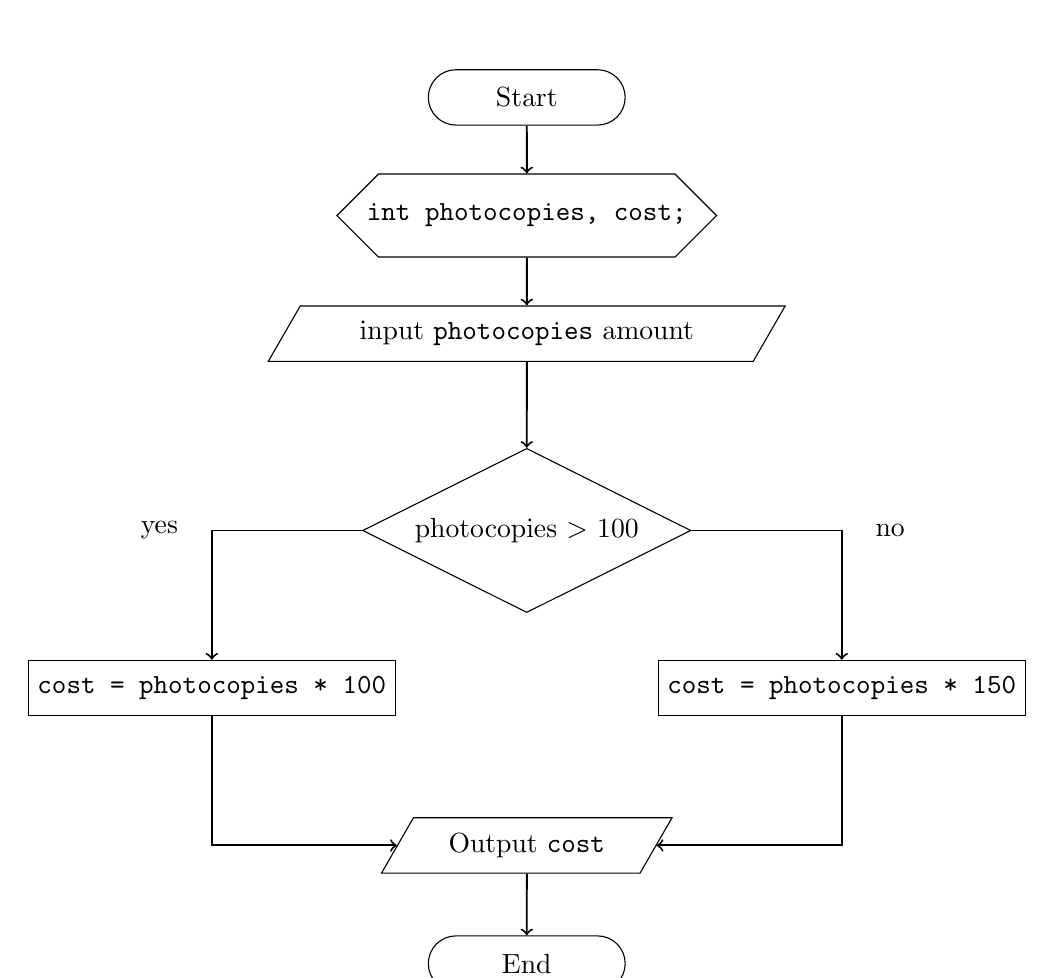
\begin{tikzpicture}
        \node (start) [terminator, align=center, minimum width=2.5cm] {Start};
        \node (prep) [preparation, below of = start, yshift = -5mm] {\texttt{int photocopies, cost;}};
        \node (input) [data, below of = prep, yshift = -5mm] {input \texttt{photocopies} amount};
        \node (branch) [decision, below of = input, yshift = -1.5cm] {photocopies $>$ 100};
        \node (calculate-gt-100) [process, below of = branch, yshift = -1cm, xshift = -4cm] {\texttt{cost = photocopies * 100}};
        \node (calculate-lt-100) [process, below of = branch, yshift = -1cm, xshift = 4cm] {\texttt{cost = photocopies * 150}};
        \node (output) [data, align=center, below of = branch, minimum width=2.5cm, yshift=-3cm] {Output \texttt{cost}};
        \node (end) [terminator, align=center, below of = output, minimum width=2.5cm, yshift=-5mm] {End};
        \draw [connector] (start) -- (prep);
        \draw [connector] (prep) -- (input);
        \draw [connector] (input) -- (branch);
        \draw [connector] (branch.west) -| node[left=3mm] {yes} (calculate-gt-100.north);
        \draw [connector] (branch.east) -| node[right=3mm] {no} (calculate-lt-100.north);
        \draw [connector] (calculate-gt-100.south) |- (output);
        \draw [connector] (calculate-lt-100.south) |- (output);
        \draw [connector] (output) -- (end);
    \end{tikzpicture}
\end{center}

\pagebreak

\section*{Assignment 2}
Indonesia Merdeka is one of the shops in Malang which is very crowded with
buyers because it is famous for the quality of the products it sells. Every
Friday, the shop gives a bonus to customers who buy Indonesian-made
electronic goods according to the total purchase.
If the total purchase from this customer is more than or equal to IDR
500.000, the bonus that the customer will get is an iron. If the total purchase
is less than IDR 500.000, the bonus the customer gets is an umbrella. Create
the flowchart!

\begin{center}
    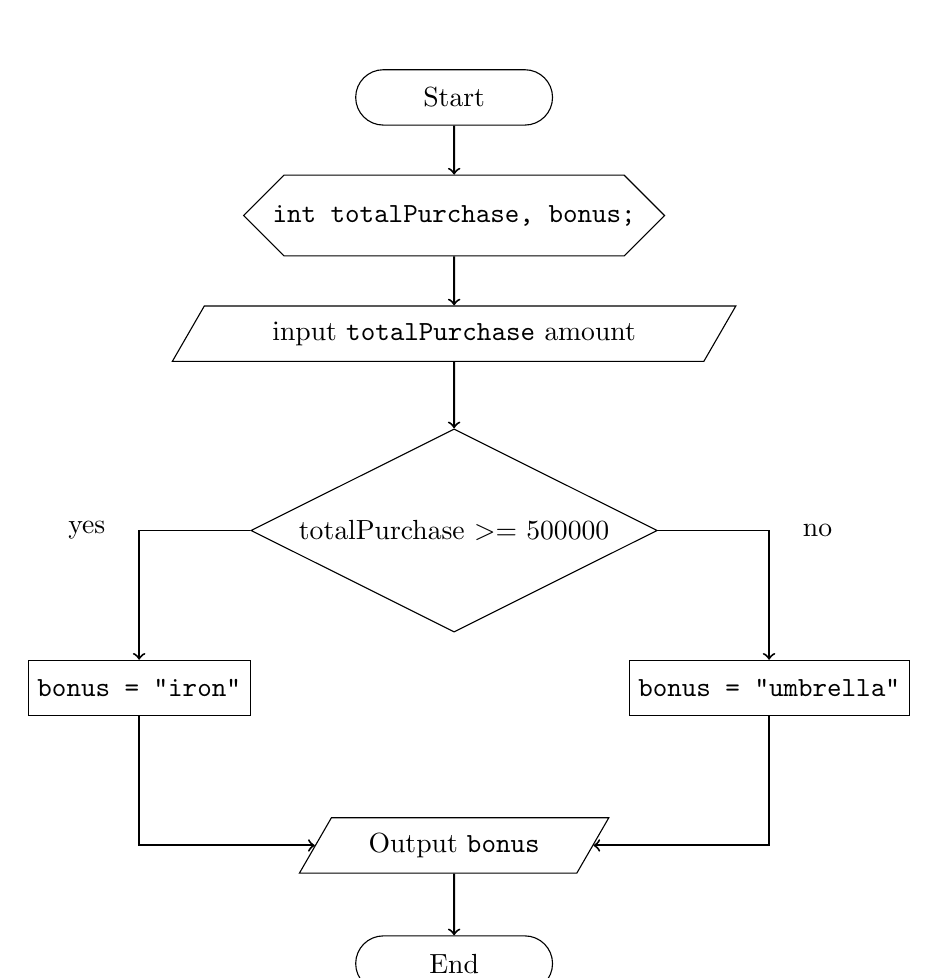
\begin{tikzpicture}
        \node (start) [terminator, align=center, minimum width=2.5cm] {Start};
        \node (prep) [preparation, below of = start, yshift = -5mm] {\texttt{int totalPurchase, bonus;}};
        \node (input) [data, below of = prep, yshift = -5mm] {input \texttt{totalPurchase} amount};
        \node (branch) [decision, below of = input, yshift = -1.5cm] {totalPurchase $>=$ 500000};
        \node (calculate-gt-100) [process, below of = branch, yshift = -1cm, xshift = -4cm] {\texttt{bonus = "iron"}};
        \node (calculate-lt-100) [process, below of = branch, yshift = -1cm, xshift = 4cm] {\texttt{bonus = "umbrella"}};
        \node (output) [data, align=center, below of = branch, minimum width=2.5cm, yshift=-3cm] {Output \texttt{bonus}};
        \node (end) [terminator, align=center, below of = output, minimum width=2.5cm, yshift=-5mm] {End};
        \draw [connector] (start) -- (prep);
        \draw [connector] (prep) -- (input);
        \draw [connector] (input) -- (branch);
        \draw [connector] (branch.west) -| node[left=3mm] {yes} (calculate-gt-100.north);
        \draw [connector] (branch.east) -| node[right=3mm] {no} (calculate-lt-100.north);
        \draw [connector] (calculate-gt-100.south) |- (output);
        \draw [connector] (calculate-lt-100.south) |- (output);
        \draw [connector] (output) -- (end);
    \end{tikzpicture}
\end{center}

\pagebreak

\section*{Assignment 3}
In a calculation program, it is known that the value of P = x + y. The user
enters two numbers x and y. After performing the calculations, if P is
positive, then the value of Q = x * y. If not, then the value Q = x / y.
Create the flowchart!
\begin{center}
    \begin{tikzpicture}
        \node (start) [terminator, align=center, minimum width=2.5cm] {Start};
        \node (prep) [preparation, below of = start, yshift = -5mm] {\texttt{int x, y, P, Q;}};
        \node (input-1) [data, below of = prep, yshift = -5mm] {input x};
        \node (input-2) [data, below of = input-1, yshift = -5mm] {input y};
        \node (process) [process, below of = input-2, yshift = -5mm] {\texttt{P = x + y}};
        \node (branch) [decision, below of = process, yshift = -1cm] {P $>$ 0};
        \node (calculate-gt-100) [process, below of = branch, yshift = -1cm, xshift = -4cm] {\texttt{Q = x * y}};
        \node (calculate-lt-100) [process, below of = branch, yshift = -1cm, xshift = 4cm] {\texttt{Q = x + y}};
        \node (output) [data, align=center, below of = branch, minimum width=2.5cm, yshift=-3cm] {Output \texttt{Q}};
        \node (end) [terminator, align=center, below of = output, minimum width=2.5cm, yshift=-5mm] {End};
        \draw [connector] (start) -- (prep);
        \draw [connector] (prep) -- (input-1);
        \draw [connector] (input-1) -- (input-2);
        \draw [connector] (input-2) -- (process);
        \draw [connector] (process) -- (branch);
        \draw [connector] (branch.west) -| node[left=3mm] {yes} (calculate-gt-100.north);
        \draw [connector] (branch.east) -| node[right=3mm] {no} (calculate-lt-100.north);
        \draw [connector] (calculate-gt-100.south) |- (output);
        \draw [connector] (calculate-lt-100.south) |- (output);
        \draw [connector] (output) -- (end);
    \end{tikzpicture}
\end{center}

\pagebreak

\section*{Assignment 4}
One form of love for the environment is throwing garbage in its place.
The following is a picture of waste bins that are differentiated based on
the type of waste to be disposed of (figure \ref{bin}). Make a flowchart to help someone
choose a waste bin when throwing garbage based on the type!

\begin{figure}[h]
    \centering
    \includegraphics[width=.5\textwidth]{images/rubbish-bin.png}
    \caption{Waste Bin}
    \label{bin}
\end{figure}

\begin{center}
    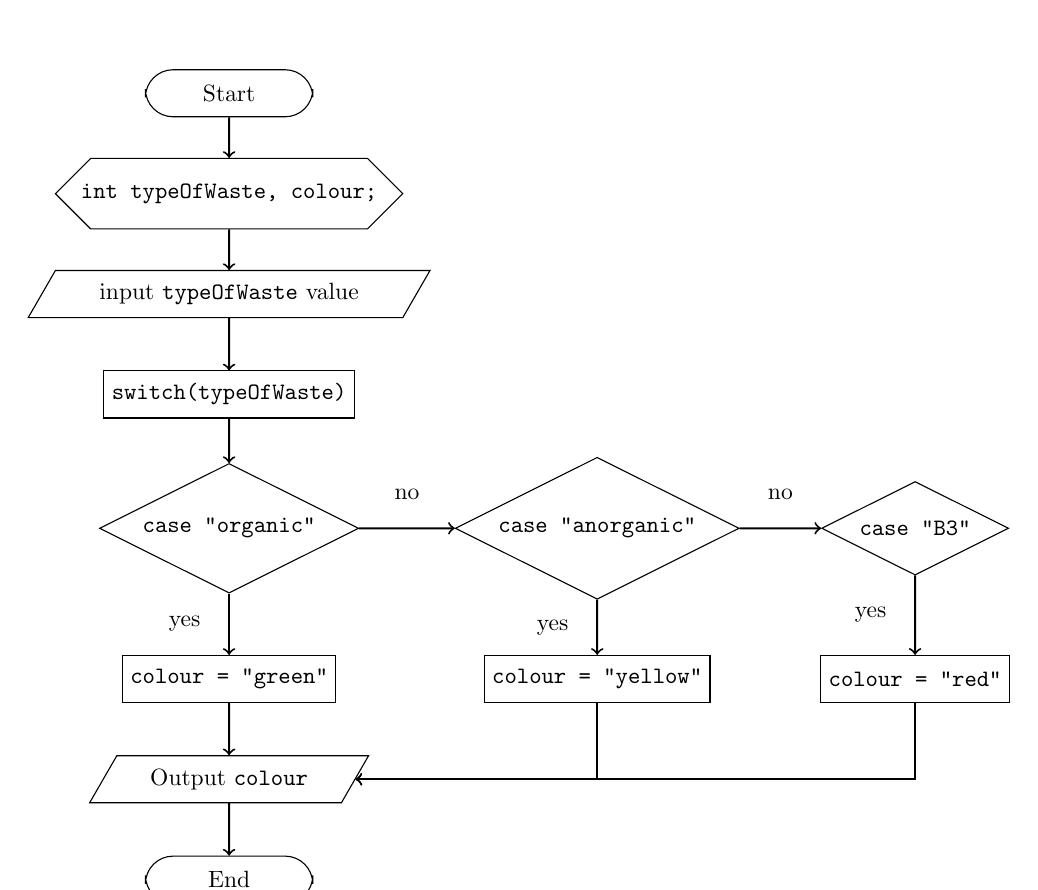
\begin{tikzpicture}[scale=0.85, every node/.style={scale=0.85}]
        \node (start) [terminator, align=center, minimum width=2.5cm] {Start};
        \node (prep) [preparation, below of = start, yshift = -5mm] {\texttt{int typeOfWaste, colour;}};
        \node (input-1) [data, below of = prep, yshift = -5mm] {input \texttt{typeOfWaste} value};
        \node (process) [process, below of = input-1, yshift = -5mm] {\texttt{switch(typeOfWaste)}};
        \node (branch-1) [decision, below of = process, yshift = -1cm] {\texttt{case "organic"}};
        \node (branch-2) [decision, right of = branch-1, xshift = 4.5cm] {\texttt{case "anorganic"}};
        \node (branch-3) [decision, right of = branch-2, xshift = 3.75cm] {\texttt{case "B3"}};
        \node (organic) [process, below of = branch-1, yshift = -1.25cm] {\texttt{colour = "green"}};
        \node (anorganic) [process, below of = branch-2, yshift = -1.25cm] {\texttt{colour = "yellow"}};
        \node (b3) [process, below of = branch-3, yshift = -1.25cm] {\texttt{colour = "red"}};
        \node (output) [data, below of = organic, yshift = -0.5cm] {Output \texttt{colour}};
        \node (end) [terminator, below of = output, align=center, minimum width=2.5cm, yshift = -0.5cm] {End};
        \draw [connector] (start) -- (prep);
        \draw [connector] (prep) -- (input-1);
        \draw [connector] (input-1) -- (process);
        \draw [connector] (process) -- (branch-1);
        \draw [connector] (branch-1.east) -- node[above=3mm] {no} (branch-2.west);
        \draw [connector] (branch-2.east) -- node[above=3mm] {no} (branch-3.west);
        \draw [connector] (branch-1) -- node[left=3mm] {yes} (organic);
        \draw [connector] (branch-2) -- node[left=3mm] {yes} (anorganic);
        \draw [connector] (branch-3) -- node[left=3mm] {yes} (b3);
        \draw [connector] (organic) -- (output);
        \draw [connector] (anorganic.south) |- (output.east);
        \draw [connector] (b3.south) |- (output.east);
        \draw [connector] (output) -- (end);
    \end{tikzpicture}
\end{center}

\end{document}
